\chapter{Components: `The Oscillator' for Adhesion and Shear-Stress Assays}
\label{Chap:Oscillator}

\section{Preface}
This chapter represents a manuscript in preparation. 

\section{Introduction}
This chapter describes the development of a modular oscillatory flow method. Although oscillatory flow could be used in a variety of ways, this component was developed to enable cell-based adhesion assays. Currently, functional cell adhesion assays are implemented using a few approaches: atomic force microscopy (AFM), micropipette manipulation, centrifugation, and fluid flow (see review \cite{Christ:2010ly}). The first two methods are intended for studying single cells and require significant expertise and are not appropriate for characterizing populations of cells. Centrifugation is simple and integrates well with a laboratory setting yet it cannot be used to interrogate aspects of dynamic cell adhesion (i.e. when the cell is attempting to adhere to a substrate in the presence of fluid flow using relatively weak, non-specific interactions) and cannot mimic physiologic fluid shear-stresses which have been shown to be important in subsequent static adhesion processes (i.e. formation of high-strength anchoring points to the substrate or cell neighbors) \cite{Sengbusch:2005zr}. Current methods that use fluid flow employ the use of spinning discs, microfluidic flow-through chambers, or simply pipetting fluid over cells. Spinning disc assays can typically only be used for studying static adhesion characteristics. Flow-through chambers employ the more physiologic phenomena of fluid shear-stress and are well-suited for microscopes to allow study of both dynamic and static adhesion events but require expensive equipment (syringe pumps, $\ge$ \$1000) to produce the fluid flow and have challenges in terms of usability due to the syringes, tubing, and fluidic connections required. Manual pipette-driven flow is simple but highly variable and the resulting data is only marginally quantitative, yet appears to be an accepted method in some areas of biology. The method presented here shares the advantages of other flow-based methods, such as the ability to study dynamic and static adhesion processes, but eliminates the costly syringe pumps and cumbersome tubes and fluidic connections. The act of connecting and maintaining tubes is replaced by the act of placing a cantilever on a membrane much like a record needle is placed to play music on a record player. The approach also allows samples to be loaded and removed using a common pipette. 

In order to validate the use of this technology in cell-based adhesion assays, the performance characteristics of the system must first be characterized. After the technical characterization, a biological validation can then be performed (see Chapter \ref{Chap:TumorCellAdhesion}). 

\section{Approach}
The device consists of a flexible PDMS diaphragm that is placed over an open microfluidic port to create a small, sealed air chamber. The diaphragm is actuated using a piezoelectric bender-actuator that responds linearly to voltage signals to induce changes in pressure that result in fluid flow.

\begin{figure}[!ht]
\centering
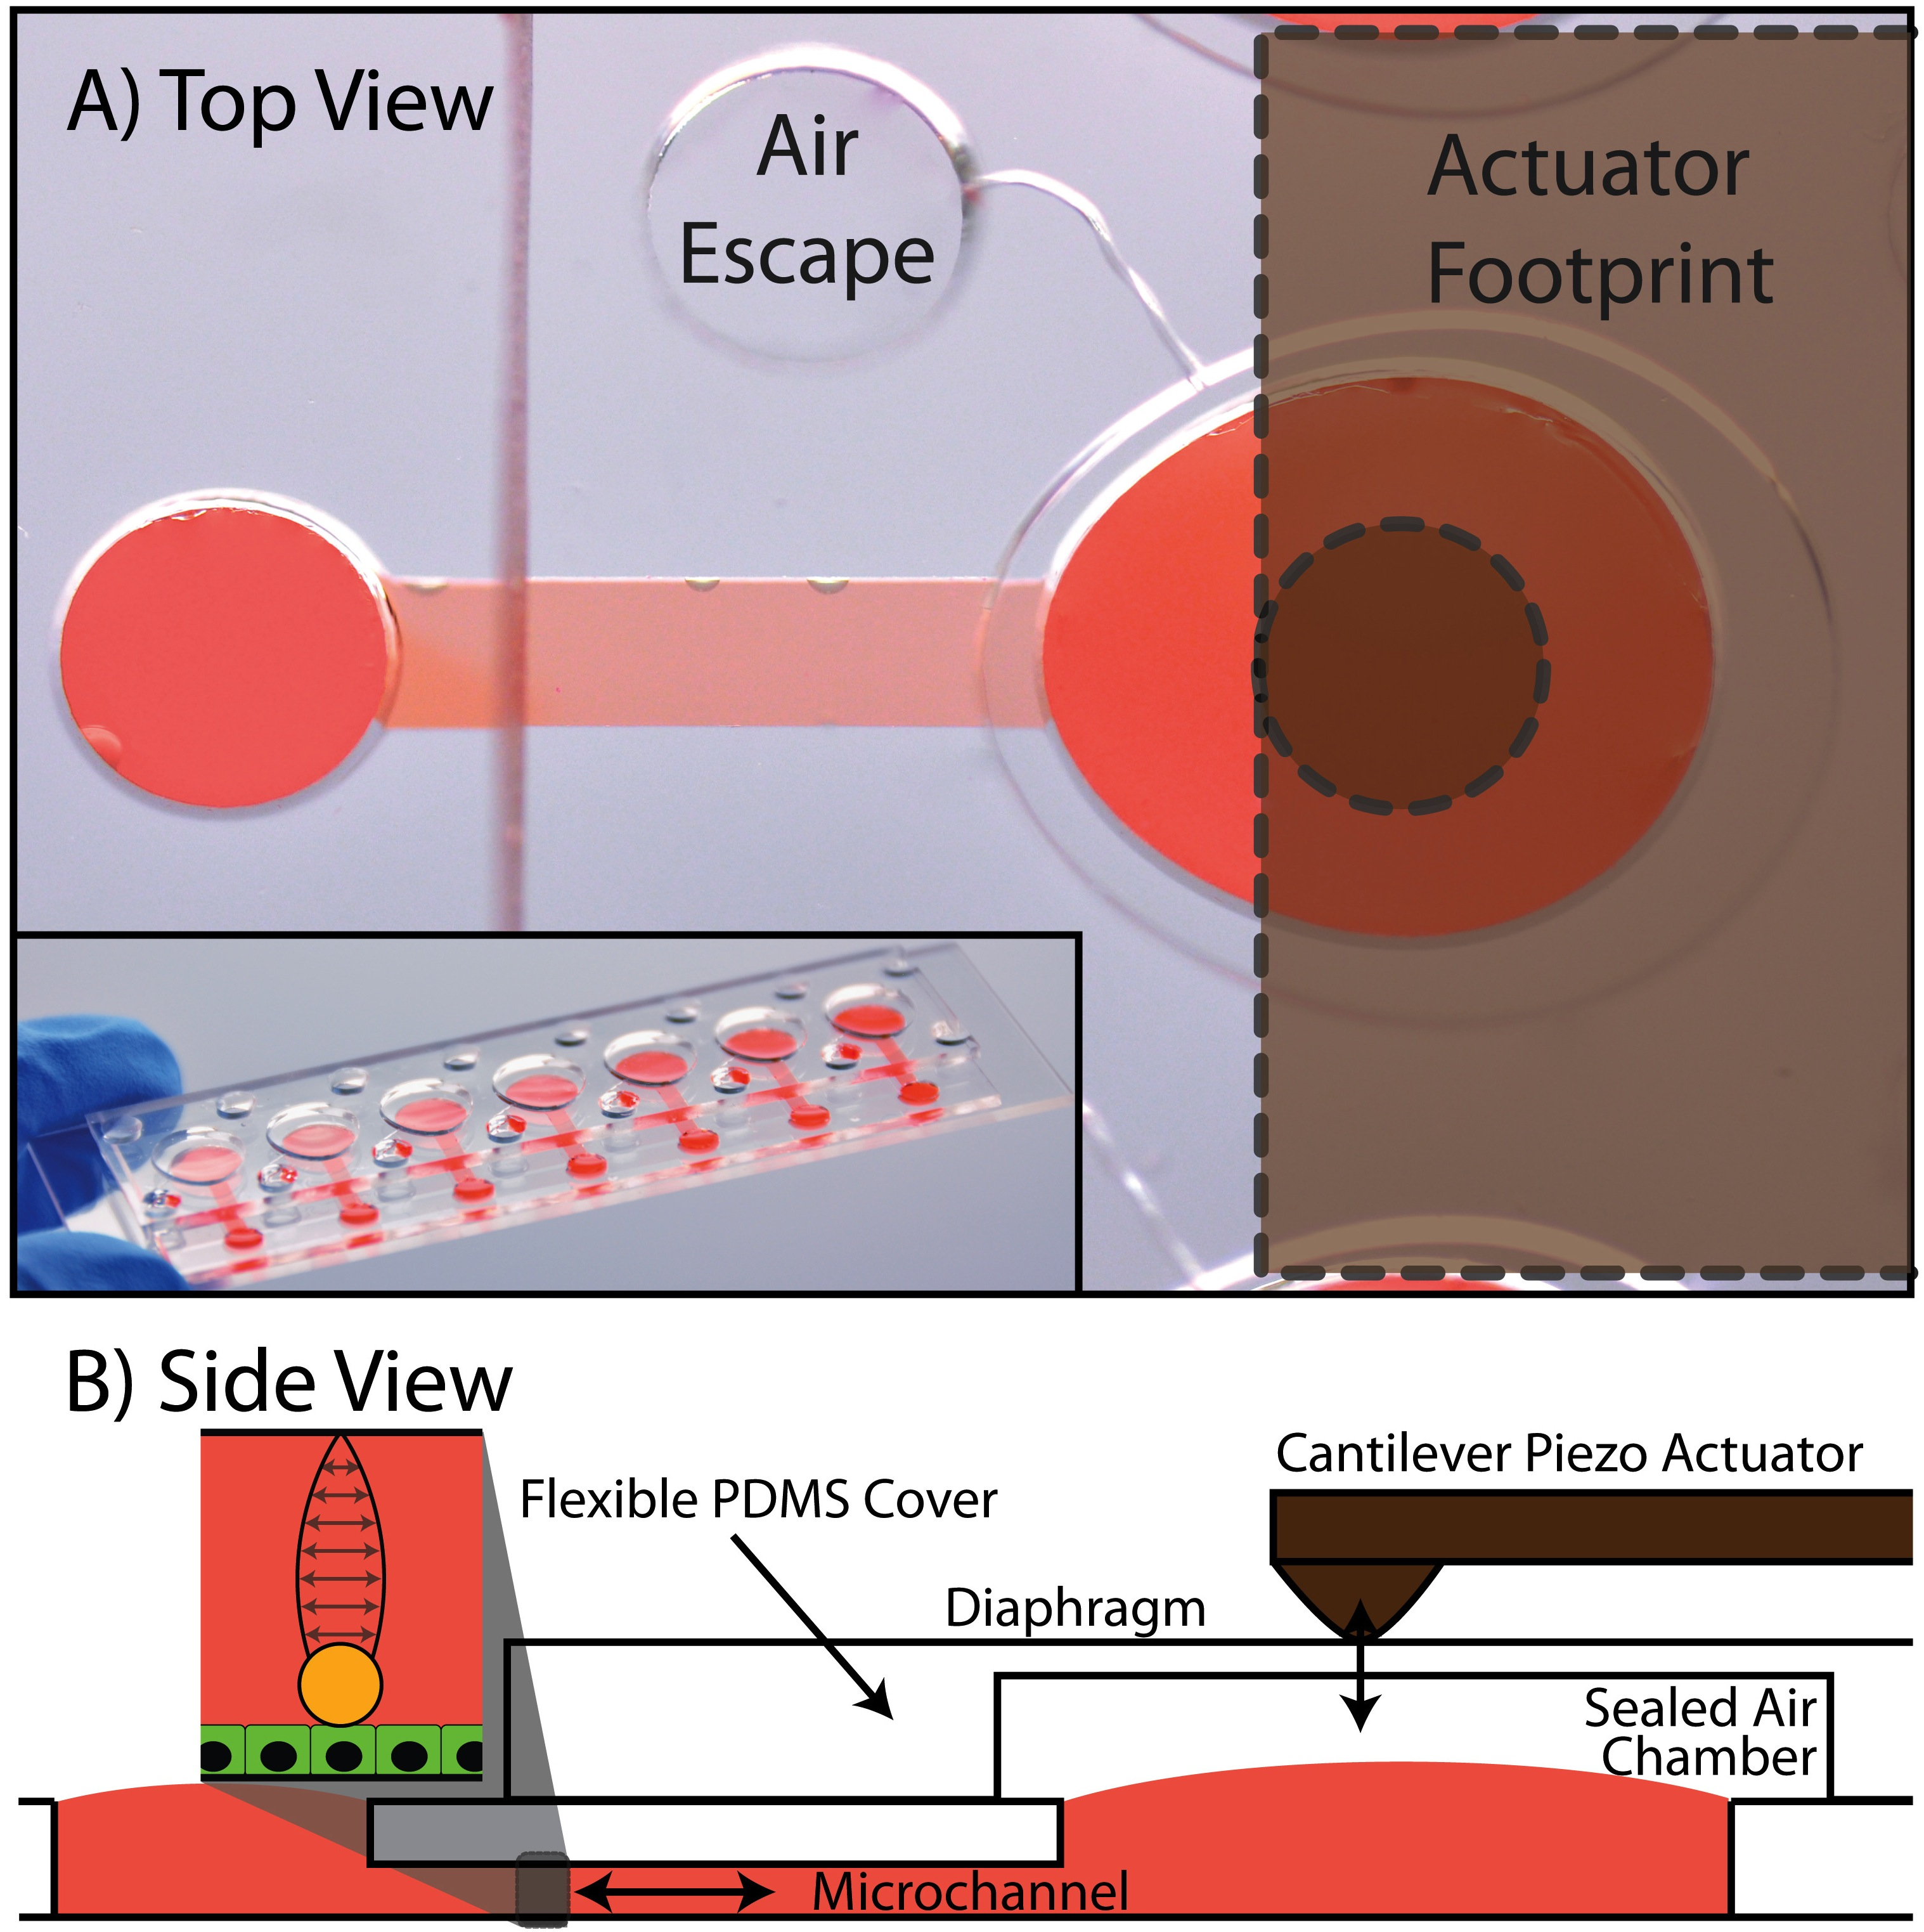
\includegraphics[width=3.5in]{OscillatoryDiagram3.jpg}
\caption{\textbf{Oscillatory flow setup}. Image of diaphragm placed over the port of a microchannel. Inset illustrates ability to array the methodology. The bender-style actuator can be made with multiple fingers or extensions to allow actuation of multiple channels at once. Similarly, the pressure at one port can be multiplexed to multiple channels.}
\label{Chap:Oscillator:Schematic}
\end{figure}

Actuation of the diaphragm was accomplished using a 3.5 cm $\times$ 1.3 cm $\times$ 0.3 cm bender-style piezo actuator (Q220-A4-303YB - Piezo Systems, Inc. Woburn, MA) with a piece of plastic and cap screw fixed to the end in order to make a focused point of contact with the diaphragm. Other non-piezo methods of actuation can be used but a piezo actuator offers the benefit of having no moving parts (\eg\, gears or ball-bearings); instead, the ceramic material bends upon application of a voltage making it more amenable to challenging environments such as incubators. A bender-style piezo actuator (flat and long like a stick of gum) is used because of the `large' range of motion that can be produced compared to other styles. One drawback of bender-actuators is that the force produced is relatively small ($<$ 1N) compared to some other designs ($>$ 1000 N). The actuator responds linearly to voltage. However the voltage levels are significantly higher than the 0-10V outputs of most signal generators. For this reason, signals are first passed through a piezo amplifier (PN: VP7206-24L105 - Viking Industrial Products. Marlboro, MA). Signals are generated using a 33220A waveform generator (Agilent Technologies Santa Clara, CA). Although a signal generator is used here, the amplifier is able to accept `mono' voltage signals coming from a headphone jack of a computer to enable simple software solutions for signal generation. Additional device setup is described in Section \ref{Chap:Oscillator:sec:methods:deviceSetup}.

\section{Characterization and Discussion}
Characterization begins with measurements of actuator response and is followed by analysis of flow within the microchannel. Given the focus here on adhesion assays, wall shear-stress is used as the primary metric of system response.

\subsection{Actuator Response}
Fig \ref{Chap:Oscillator:fig:actuatorResponse} shows how the actuator responds to voltage as well as its frequency-response. These tests were performed using the fully assembled actuator and tip but without being in contact with the diaphragm.  The actuator voltage-response was linear while the frequency response illustrates constant amplitudes below 20 Hz and a resonant frequency that was greater than 80 Hz.

\begin{figure}[!b]
\centering
\begin{tabular}{p{0.3cm}cp{0.3cm}c}
A) & \imagetop{\includegraphics[width = 2.5in]{PizeoVoltageResponse.pdf}} & B) &
\imagetop{\includegraphics[width = 2.5in]{PiezoFrequencyResponse.pdf}}\cr
\end{tabular}
\caption{\textbf{Voltage and frequency response of piezoelectric bender-actuator}. A) Actuator amplitude is linear to the input voltage. B) Actuator amplitude was constant below 16 - 32 Hz. The resonant frequency is $>$ 80 Hz.}
\label{Chap:Oscillator:fig:actuatorResponse}
\end{figure}

It is expected that coupling of the actuator with the microchannel and membrane will alter the frequency response, likely damping the resonance observed at high frequencies.

\subsection{Shear-Stress Response}
Excluding the frequency response of the actuator, there are two characteristic frequencies of this diaphragm-microchannel setup. The first dictates the transition from quasi-steady flow to pulsatile flow while the second marks a transition in the behavior of the pumping mechanism from being much like a syringe pump to being like a regulated pressure source. These transitions are discussed more fully in the next two sections.

\subsubsection{Flow Transition: Quasi-steady \vs\ Pulsatile}
The Womersley number can be used to help characterize the pulsatile nature of the flow (Eq \ref{Chap:Oscillator:equ:womersley}) as it provides a measure of the balance between viscosity and momentum effects induced by oscillatory motion. 

\begin{equation}
\Omega = a \sqrt{\frac{2 \pi f \rho}{\mu}}
\label{Chap:Oscillator:equ:womersley}
\end{equation}
 
In Appendix \ref{App:Oscillator}, it is shown that the critical value for the Womersley number in PPFCs is 2.8 where the height of the PPFC is used as the critical length dimension, $a$. The dimensions of the simple one-input-one-output channel used in these studies are L $\times$ W $\times$ H = 7.5mm $\times$ 1.5 mm $\times$ 0.228 mm. Given these channel dimensions, previous work by Bacabac \etal\ suggests that the shear-stress will remain linear with pressure-gradient below 4.8 Hz. This can be seen in Fig \ref{Chap:Oscillator:fig:flowTransition} where pulsatile-flow shear-stress is normalized by steady-flow shear-stress calculated using the same pressure gradient. At low frequencies, the two models predict the same shear-stress whereas the pulsatile model attenuates above the transition frequency. Shear-stress attenuates due to inertial effects induced by high frequency oscillations.

\begin{figure}[!ht]
\centering
\includegraphics[width=3.5in]{Pulsatile_vs_SteadyShear2.pdf}
\caption{\textbf{Transition from steady to pulsatile flow}. The influence of non-parabolic flow profiles can be seen on shear-stress for frequencies above the transition frequency of 4.8 Hz. This simulation keeps pressure constant while varying frequency. Shear stress is normalized to the shear stress measured at the lowest frequency, which is nearly identical to the steady-flow solution for the same pressure gradient.}
\label{Chap:Oscillator:fig:flowTransition}
\end{figure}

\subsubsection{Pumping Transition}
The ports and air chamber of the oscillatory flow setup act as capacitors with the microchannel acting as a resistance between them. At low frequencies, the capacitors are negligible and the volume displaced in the channel is equal to the volume of air displaced by the actuator\slash diaphragm. At high frequencies, the resistance of the channel impedes charging and discharging of the capacitors, leading to a situation where fluid displacement is less than the air displaced by the actuator\slash diaphragm. This can be seen in a plot of simulation results (for methods see Section \ref{Chap:Oscillator:sec:methods:shear}) where the ratio of the air displaced by the diaphragm is compared to the fluid displacement in the channel for a range of frequencies (Fig \ref{Chap:Oscillator:fig:pumpingTransition}). At low frequencies, the pumping mechanism behaves much like a syringe pump and falls rapidly when above a certain cutoff frequency. This transition in the pumping behavior can be roughly estimated by calculating the capacitance of the air chamber ($C = $3.8e-13 [m$^{3}$/Pa]) and the resistance of the microchannel ($R = $3.95e9 [Pa-s/m$^{3}$]). The characteristic frequency of the transition can then be calculated using an RC-circuit analogy where $f = 1/(2\pi RC) = 106$ Hz, which represents the frequency at which signal should be attenuated by roughly half. This calculation agrees very well with the simulation results. Although the transition is predicted to be near 106 Hz, the initial effects of the transition can be seen earlier, at $\sim$ 30 Hz. Still, the pumping transition frequency is well above the flow transition frequency; thus, the range where shear-stress increases linearly with frequency is limited by the physics of pulsatile flow within the microchannel rather than the pumping mechanism. The pumping transition frequency can be increased if necessary by reducing the volume in the air-chamber to create a stiffer capacitor (\ie\, lower capacitance).

At extremely high frequencies, the fluid displacement will be negligible compared to the air-volume displaced by the actuator\slash diaphragm, resulting in what behaves like a pressure-based pump rather than a volume-based pump like a syringe-pump where all lines are completely filled with fluid.

\begin{figure}[!ht]
\centering
\includegraphics[width=3.5in]{ChannelFrequencyResponseTheory2.pdf}
\caption{\textbf{Transition from syringe-pump-like behavior to pressure-driven behavior}. Normalized volume displacement represents the ratio of the air-volume displaced by the actuator to the volume of fluid displaced in the channel. Simulation suggests that at low frequencies, the air and fluid displacement are tightly coupled with a ratio of almost 1. At higher frequencies, the capacitance of the air chamber coupled with the resistance of the microchannel result in a coupling that is less than 1, approaching 0 when $f \gg 106 Hz$.The capacitance of the air chamber and resistance of the channel suggest a pumping transition frequency of roughly 100 Hz which coincides with simulation results.}
\label{Chap:Oscillator:fig:pumpingTransition}
\end{figure}


\subsubsection{Overall System Response}
Overall System response was measured experimentally to observe change in shear-stress with respect to both frequency and actuator amptlitude\slash voltage

\begin{figure}[!ht]
\centering
\includegraphics[width=3.5in]{ChannelFrequencyResponse.pdf}
\caption{\textbf{Channel frequency response}. }
\label{Chap:Oscillator:fig:channelFrequencyResponse}
\end{figure}

Fig \ref{Chap:Oscillator:fig:channelFrequencyResponse} shows the frequency response at an actuator voltage of 100 mV. Experimental measurements of shear-stress were obtained from observations of particle motion as described in Section \ref{Chap:Oscillator:sec:methods:shear}. As predicted in the previous discussions of the flow and pumping transition frequencies, shear-stress is linearly related to frequency below 5 Hz. Above 5 Hz, the influence of non-parabolic flow profiles and air-chamber capacitance can be seen to influence the linear relationship.

In Fig \ref{Chap:Oscillator:fig:channelVoltageResponse}, shear-stress was measured in the channel across a range of voltages for three different frequencies (for methods see Section \ref{Chap:Oscillator:sec:methods:shear}). Shear-stress changed linearly with voltage at each frequency. Measurement variability increases with frequency and voltage given the measurement method used here. Acoustic streaming increases with frequency and induces particle motion that makes it more difficult to determine amplitude in the center streamline. Similarly, at high voltages, it can be difficult to observe a full oscillation of particle motion in one field of view of the microscope camera. The linear behavior is expected given the linear relationship between pressure-gradient and shear-stress in the equations outlined in Appendix \ref{App:Oscillator} for pulsatile flow.

\begin{figure}[!ht]
\centering
\includegraphics[width=3.5in]{ChannelVoltageResponse.pdf}
\caption{\textbf{Channel voltage response}. Shear-stress is measured across a range of piezo voltages for three different frequencies. Each series of points indicates linear relation ship between shear-stress and voltage, which is in agreement with simulation as well (see App \ref{App:Oscillator}).}
\label{Chap:Oscillator:fig:channelVoltageResponse}
\end{figure}

\section{Methods}
\subsection{Actuator Motion Measurements}
Motion was measured using bright-field microscopy where the actuator was mounted on its side such that the tip appeared to move side-to-side in the field of view. Motion was quantified from digital images.

\subsection{Fluid Flow Modeling and Shear-Stress Estimation}\label{Chap:Oscillator:sec:methods:shear}
The microfluidic channel was approximated as a parallel-plate flow-chamber (PPFC). Fluid flow was modeled using methods for both steady-flow and pulsatile-flow where flow is laminar. Modeling of the flow transition frequency utilized the pulsatile flow model whereas modeling of the pumping transition frequency used the steady flow model. The steady flow model is needed in this case in order to separate effects of flow transition from pumping transition. These equations for steady and pulsatile flow are given in Appendix \ref{App:Oscillator}. 

Fig \ref{Chap:Oscillator:fig:amplitudeMeasurements} compares the use of a steady and pulsatile model of flow for determining shear-stress from particle amplitude. In this graph, the magnitude of the pressure gradient is held constant while frequency is changed. For each frequency, the pulsatile model is used to determine the amplitude of the fluid motion in the center streamline. This amplitude is then used in the steady-flow equation for determining shear-stress from particle amplitude (Appendix \ref{App:Oscillator}). The results show that the amplitude of the fluid motion can be used to predict shear-stress using an assumption of a parabolic flow profile with $<$ 5\% below 32 Hz and $<$ 1\% below 13.8 Hz. This helps to make estimation of shear-stress from measured particle-amplitudes a much easier calculation for experimentation. However, given the pulsatile model is in place, the pulsatile model was used for all experimental measurements.

\begin{figure}[!ht]
\centering
\includegraphics[width=3.5in]{Pulsatile_vs_SteadyShear.pdf}
\caption{\textbf{Shear-stress from particle amplitude}. (solid-black) Shear-stress is plotted \vs\ frequency using the pulsatile model of flow in a PPFC. (dotted) The dotted line indicates the shear-stress that would be predicted if one were to measure particle amplitude in the channel and use a parabolic flow profile assumption to predict the shear-stress. (solid-gray) The solid-gray line indicates the error relative to the non parabolic line. Error is plotted at the same scale as normalized shear-stress with potential values between 0 and 1. The error line suggests error is $<$ 5\% below 32 Hz and $<$ 1\% below 13.8 Hz.}
\label{Chap:Oscillator:fig:amplitudeMeasurements}
\end{figure}

Shear-stress was estimated using particle motion. Particle motion was measured using 15 \textmu m fluorescent beads (PN:F8843 - Invitrogen. Eugene, OR) on an inverted fluorescent microscope (PN:IX70 - Olympus. Center Valley, PA) equipped with a digital camera (PN:C4742-80-12AG - Hamamatsu, Hamamatsu City, Japan) and MetaMorph imaging software (Molecular Devices. Sunnyvale, CA). While oscillating the particles, the channel was flipped upside-down to cause the beads to settle to the ceiling of the microchannel. This was done while actuating the channel. After 1.5 min, the channel was placed rightside-up on the microscope. The exposure time for each image was set to capture at least one full cycle of bead motion in a single image, making the bead appear as a streak. The images were captured in rapid succession using the `Acquisition Stream' function of MetaMorph to record particle amplitude as it settled from the ceiling to the substrate. Roughly 30 images are acquired during settling providing ample opportunity to select a frame in which a bead near the center portion of the channel reaches its maximum amplitude. The pixel length of the streak is recorded and converted to an amplitude in meters which is then converted to a shear-stress in Pa using a pulsatile model of flow to relate amplitude with shear-stress.

This method of shear-stress determination becomes more challenging at high frequencies and amplitudes. At high amplitudes, the entire particle motion can extend beyond the view-field of the camera. At high frequencies acoustic streaming can occur near device edges and bubbles to disturb cell settling and make it difficult to ensure the particle is traveling through a position where it will exhibit its maximum displacement \cite{Chung:2008fk}. Also, at high enough frequencies, the maximum fluid-displacement does not occur at the center streamline. Although not quantified here, it is estimated that this effect could be noticed in the image sequences at frequencies above 20 Hz. Although challenges in shear-stress determination can occur at high amplitudes and frequencies, overall, the method is repeatable (see Fig \ref{Chap:Oscillator:fig:channelFrequencyResponse}), fast, and appropriate for channel calibration in adhesion assays where physiological frequencies are $\sim$ 1 Hz and attachment occurs at shear-stresses $<$ 1 Pa. In roughly 2 minutes, the shear-stress in the channel can be determined and repeated to within a couple pixels.

\subsection{Device Setup}\label{Chap:Oscillator:sec:methods:deviceSetup}
The microchannel and diaphragm design are illustrated in Fig \ref{Chap:Oscillator:fig:deviceDesign}. The components were made from polydimethylsiloxane (PDMS).

\begin{figure}[!ht]
\centering
\includegraphics[width=1.5in]{MicrochannelDesign.pdf}\hspace{0.5cm}\includegraphics[width=1.5in]{DiaphragmDesign.pdf}
\caption{\textbf{Device design}. Microchannel: 0.228 mm $\times$ 1.5 mm $\times$ 7.5 mm (from inside edge of input to inside edge of output). Channel input port: 1.5 mm radius. Channel output port: 6.24 mm $\times$ 5.6 mm. Air chamber: 7 mm $\times$ 7.8 mm $\times$ 1 mm. Air escape channel: 50 \textmu m tall $\times$ 100 \textmu m wide. Air escape port: 3 mm radius. The diaphragm is the ceiling of the air chamber. The thickness of the diaphragm is determined by the difference in thickness between the air chamber feature an air escape port, which is estimated to be 250 \textmu m.}
\label{Chap:Oscillator:fig:deviceDesign}
\end{figure}


The PDMS microchannel devices were first placed in OmniTrays (Thermo Fisher Scientific. Rochester, NY) and filled with PBS containing 0.5\% BSA to discourage beads from sticking to each other or the walls of the device. The diaphragm is placed over the large port of the device while leaving the small port exposed to the atmosphere. The air escape allows fluid to be loaded while the diaphragm is already in place. Without the air escape, fluid cannot be loaded efficiently due to the relative capacitance of the exposed port and sealed air chamber.

Within the OmniTray, a metal strip is fixed to the bottom using double-sided tape. The actuator, mounted to a 1 cm $\times$ 2.5 cm piece of plastic via double-sided tape is held in place on the metal strip with magnets fixed to the actuator assembly. This provided an easy means to place and remove the actuator. The position of the actuator was able to remain very stable during manipulation of the OmniTray, enabling the flip technique for shear estimation. The cap screw used as the point of contact between the actuator and diaphragm provided height adjustability where needed. The entire assembly could be enclosed in a covered OmniTray. The lid provided enough compliance for the small wires leading to the piezo-actuator.

The actuator is placed on the diaphragm just prior to experimentation but can be put in place earlier if desired. The voltage and frequency of oscillation are set and the beads are loaded. After loading, the air escape is plugged using a drop of bead suspension or other fluid that will pin at the entrance to the air escape port.

Immediately after loading, the microscope is focused on the beads and the entire OmniTray is flipped and placed on a surface to remain level for 1.5 min to allow the beads to settle to the ceiling for subsequent imaging. After each set of images, the OmniTray is flipped again to reset the beads to the ceiling and allow for a repeat of the measurement. 

\section{Other Potential Applications}
Although the device is aimed at use for performing cell-based adhesion and shear-stress assays, the oscillatory pressure source could be used of other things as well. For example, the oscillating pressure can be rectified to produce net flow in one direction or recirculatory flow\cite{Leslie:2009vn,Seker:2009uq}. It has also been shown that the oscillatory nature of pumps can be used with high and low pass filters to produce tunable `valving' for other behavior within a device\cite{Mosadegh:2010kx}. Also, the oscillating air pressure can be used as well to drive fluid in other ways\cite{Langelier:2009qm}. Given the lack of moving or rusting parts, the method is also amenable to prolonged exposure within incubators for long-term application of shear-stress.

\section{Conclusions}
A tubeless method for producing oscillatory flow in microchannels has been presented. The method addresses various shortcoming of other methods to provide a tubeless method method for producing quantifiable oscillatory shear-stress in a microchannel that can be addressed using a pipette or liquid handling automation. The device analyzed here shows a linear shear-stress response to changes in frequency below 5 Hz but is capable of providing complex signals with much higher harmonics (up to $\sim$ 30 Hz) with the understanding that non-parabolic flow profiles and inertial considerations begin to add non-linearity to the response. Two characteristic frequencies determine the behavior of the device, the flow transition frequency, dictated by the Womersley number, and the pumping transition frequency, dictated by the resistance of the microchannel and dimensions of the air chamber. Transition between quasi-steady and pulsatile flow occurred near 5 Hz while the pumping transition frequency was estimated to be near 100 Hz suggesting syringe-pump-like behavior below 30 Hz.






